\documentclass[a4paper, utf8]{ctexart}
\usepackage[fontset=Fandol]{ctex}
\usepackage{anyfontsize}
\usepackage{algorithm}
\usepackage{abstract}
\usepackage{amsfonts}
\usepackage{appendix}
\usepackage{booktabs}
\usepackage{enumitem}
\usepackage{fancyhdr}
\usepackage{geometry}
\usepackage{graphicx}
\usepackage{tabularx}
\usepackage{listings}
\usepackage{amsmath}
\usepackage{caption}
\usepackage{lipsum}
\usepackage{minted}
\usepackage{xcolor}
\usepackage{array}

\geometry{a4paper,left=31mm,right=31mm,top=25mm,bottom=25mm}
\CTEXsetup[format={\Large \bfseries}]{section}

\setlength{\parindent}{2em}
\pagestyle{fancy}
\fancyhf{}
\fancyhead[L]{并行程序设计与算法实验\ 实验报告}
\fancyhead[R]{Lab0\ 环境设置与串行矩阵乘法}
\fancyhead[C]{}
\fancyfoot[C]{\thepage}
\fancyfoot[L,R]{}

\setCJKfamilyfont{zhsong}[AutoFakeBold = {2.17}]{SimSun}
\renewcommand*{\songti}{\CJKfamily{zhsong}}
\definecolor{LightGray}{gray}{0.9}

\title{\songti \bfseries Lab0\ 环境设置与串行矩阵乘法}
\author{\fangsong 21307210\ \ 傅祉珏}
\date{\fangsong 中山大学计算机学院\ 广东广州\ 510006}

\begin{document}
	
	\begin{titlepage}
		\centering
		\rule{\textwidth}{1pt}
		\vspace{0.02\textheight}
		
		{\LARGE \kaishu 并行程序设计与算法实验\ 实验报告}
		
		\vspace{0.02\textheight}
		
		{\Huge \songti \bfseries Lab0\ 环境设置与串行矩阵乘法}
		
		\vspace{0.025\textheight}
		\rule{0.83\textwidth}{0.4pt}
		\vspace{0.05\textheight} 
		\begin{figure}[htbp]
			\centering
			
\includegraphics[width=8cm, height=8cm]{./figure/计院院徽.jpg}
		\end{figure}
		
		\vspace{0.04\textheight} 
		{\Large 姓名:傅祉珏}
		
		\vspace{0.025\textheight} 
		{\Large 学号:21307210}
		
		\vspace{0.025\textheight} 
		{\Large 专业:计算机科学与技术}
		
		\vspace{0.025\textheight} 
		{\Large Email:futk@mail2.sysu.edu.cn}
		
		\vspace{0.025\textheight} 
		{\Large 完成时间:\today}
		
		\vspace{0.05\textheight} 
		\vfill
		
		{\large \today}
		\vspace{0.1\textheight}
		\rule{\textwidth}{1pt}
	\end{titlepage}
	\let\cleardoublepage\clearpage
	
	\maketitle
	
	\renewcommand{\abstractname}{\large \textbf{摘要}}
	\begin{abstract}
		本实验针对矩阵乘法的计算效率优化进行了系统研究,探索了从基础串行实现到多层次优化的过程。实验分析了朴素三重循环矩阵乘法的性能瓶颈,并通过调整循环顺序(ikj 变换)、编译优化(-O3 选项)、并行化(OpenMP)、分块矩阵乘法、自动向量化及 Intel MKL 库优化等多种策略,提升了计算效率。实验结果表明,编译优化能减少指令执行开销,并行化能充分利用多核资源,分块矩阵乘法提升了缓存利用率,而 MKL 库优化则接近理论峰值性能。最终,实验验证了不同优化方法的有效性,并为进一步研究 GPU 加速(CUDA、OpenCL)及混合并行计算(MPI + OpenMP)提供了参考。
		
		\noindent{\textbf{\heiti 关键词:}矩阵乘法优化,OpenMP,并行计算,缓存优化,Intel MKL。}
	\end{abstract}
	
	\section{实验目的}
	
	在软件开发过程中,提升程序性能是一个至关重要的任务,被称为性能工程(Performance Engineering)。性能工程旨在优化低效代码,并根据硬件架构定制软件,以提高计算效率和资源利用率。为了深入理解性能工程的目标和方法,本实验将针对朴素矩阵乘法算法进行优化分析与实现。
	
	在数学领域中,一个 $m \times n$ 维矩阵是由 $m$ 行 $n$ 列元素组成的矩形数组。矩阵运算是数值计算与科学计算中的核心问题,并在统计分析、计算机图形学和机器学习等诸多应用领域中发挥重要作用。通用的矩阵乘法运算由以下数学表达式定义:
	
	\vspace{-.75em}
	\begin{equation}
		C_{i,j} = \sum_{p=1}^{k} A_{i,p} \cdot B_{p,j}	\nonumber
	\end{equation}
	
	其中,矩阵 $A$ 维度为 $m \times k$,矩阵 $B$ 维度为 $k \times n$,其乘积矩阵 $C$ 的维度为 $m \times n$。矩阵 $C$ 的元素 $C_{i,j}$ 由矩阵 $A$ 的第 $i$ 行向量与矩阵 $B$ 的第 $j$ 列向量的内积计算得到。
	
	本实验的主要目标是从多个维度优化矩阵乘法计算,包括算法优化、数据存取优化以及硬件加速等方面,以提升计算效率并获得优化后的性能表现。
	
	\section{实验过程}
	
	本实验围绕串行矩阵乘法的优化展开,依次实现并分析不同优化方法对计算性能的影响。
	
	\subsection{朴素串行矩阵乘法实现}
	
	在未进行优化的情况下,矩阵乘法通常采用三重循环的方式进行计算。设有矩阵 $A$($m \times k$ 维)与矩阵 $B$($k \times n$ 维),计算其乘积矩阵 $C$($m \times n$ 维)时,基本实现如下:
	
	\begin{minted}[baselinestretch=1, framesep=0mm, escapeinside=||]{cpp}
for (int i = 0; i < N; i++) {
    for (int j = 0; j < N; j++) {
        double sum = 0.0;
        for (int k = 0; k < N; k++) {
            sum += A[i * N + k] * B[k * N + j];
        }
        C[i * N + j] = sum;
    }
}
	\end{minted}
	
	该实现按照 $i-j-k$ 顺序遍历矩阵,逐元素计算内积。由于该方法没有针对缓存优化,存在大量的缓存未命中(cache miss)现象,导致性能较低。
	
	\subsection{调整循环顺序优化(ikj 循环顺序)}
	
	为了提高缓存利用率,本实验首先调整循环顺序为 $i-k-j$,即:
	
	\begin{minted}[baselinestretch=1, framesep=0mm, escapeinside=||]{cpp}
for (int i = 0; i < N; i++) {
    for (int k = 0; k < N; k++) {
        double a = A[i * N + k];
        for (int j = 0; j < N; j++) {
            C[i * N + j] += a * B[k * N + j];
        }
    }
}
	\end{minted}
	
	这种方式的优化原理在于,在外层循环固定行索引 $i$ 和中间层循环固定列索引 $k$ 后,矩阵 $B$ 的访问模式变为按列访问,提高了数据局部性,同时减少了缓存未命中率。
	
	\subsection{编译优化}
	
	接下来,利用编译器优化选项进一步提升计算效率。例如,在 gcc 编译 C++ 代码时,可以使用如下命令启用优化:
	
	\begin{minted}[baselinestretch=1, framesep=0mm, escapeinside=||]{bash}
g++ -O3 -march=native test5 test5.cpp
	\end{minted}
	
	编译优化的核心作用在于启用循环展开(loop unrolling)、指令重排(instruction reordering)以及自动向量化(auto-vectorization)等优化策略,以减少指令开销,提高执行效率。
	
	\subsection{并行化优化}
	
	在单线程串行计算的基础上,使用 OpenMP 实现多线程并行计算,利用多核 CPU 资源加速计算。例如,将最外层循环并行化:
	
	\begin{minted}[baselinestretch=1, framesep=0mm, escapeinside=||]{cpp}
#pragma omp parallel for  // |并行化外层|i|循环|
for (int i = 0; i < N; i++) {
    for (int k = 0; k < N; k++) {
        double a = A[i * N + k];
        for (int j = 0; j < N; j++) {
            C[i * N + j] += a * B[k * N + j];
        }
    }
}
	\end{minted}
	
	OpenMP 并行化能够充分利用多核处理器的计算能力,提高计算吞吐量,但可能会带来线程同步开销,因此需要合理设定线程数,以获得最佳性能。
	
	\subsection{分块矩阵乘法优化}
	
	为了进一步优化缓存利用率,采用分块矩阵乘法(Blocked Matrix Multiplication)策略,将矩阵划分为小块并逐块进行计算,以提高数据局部性。其核心代码如下:
	
	\begin{minted}[baselinestretch=1, framesep=0mm, escapeinside=||]{cpp}
const int BLOCK_SIZE = 64;  // |分块大小(根据|CPU|缓存调整)|
#pragma omp parallel for collapse(2)  // |外层双循环并行|
for(int i = 0; i < N; i += BLOCK_SIZE) {
    for(int j = 0; j < N; j += BLOCK_SIZE) {
        for(int k = 0; k < N; k += BLOCK_SIZE) {
            for(int il = 0; il < BLOCK_SIZE; il ++) {
                for(int kl = 0; kl < BLOCK_SIZE; kl ++) {
                    for(int jl = 0; jl < BLOCK_SIZE; jl ++) {
                        C[(i + il) * N + (j + jl)] += A[(i + il) * N + (k + kl)]
                                                    * B[(k + kl) * N + (j + jl)];
                    }
                }
            }
        }
    }
}
	\end{minted}
	
	该优化方法利用了缓存行(cache line)的空间局部性,提高了缓存命中率,从而减少访存开销,提高计算性能。
	
	\subsection{自动向量化优化}
	
	自动向量化(Auto-Vectorization)是编译器级优化,能够利用 SIMD 指令集(如 AVX、SSE)实现并行计算。通常,编译器会在高优化级别(如 -O3)下自动启用向量化,但可以通过 \#pragma 指令显式提示编译器优化:
	
	\begin{minted}[baselinestretch=1, framesep=0mm, escapeinside=||]{cpp}
const int BLOCK_SIZE = 64;  // |分块大小(根据|CPU|缓存调整)|
#pragma omp parallel for collapse(2)  // |外层双循环并行|
for(int i = 0; i < N; i += BLOCK_SIZE) {
    for(int j = 0; j < N; j += BLOCK_SIZE) {
        for(int k = 0; k < N; k += BLOCK_SIZE) {
            #pragma omp simd
            for(int ii = 0; ii < BLOCK_SIZE; ii ++) {
                for(int kk = 0; kk < BLOCK_SIZE; kk ++) {
                    for(int jj = 0; jj < BLOCK_SIZE; jj ++) {
                        C[(i + ii) * N + (j + jj)] += A[(i + ii) * N + (k + kk)]
                                                    * B[(k + kk) * N + (j + jj)];
                    }
                }
            }
        }
    }
}
	\end{minted}
	
	向量化能够并行处理多个数据元素,有效提升计算吞吐率,但依赖于硬件 SIMD 支持以及编译器的优化能力。
	
	\subsection{手工 AVX 向量化}
	
	相比自动向量化,手工 AVX 优化能够更精细地控制 SIMD 指令的执行,以进一步提升性能。例如,使用 AVX 指令集进行矩阵乘法优化如下:
	
	\begin{minted}[baselinestretch=1, framesep=0mm, escapeinside=||]{cpp}
const int BLOCK_SIZE = 64;
#pragma omp parallel for collapse(2)
for (int i = 0; i < N; i += BLOCK_SIZE) {
    for (int j = 0; j < N; j += BLOCK_SIZE) {
        for (int k = 0; k < N; k += BLOCK_SIZE) {
            for (int ii = i; ii < min(i + BLOCK_SIZE, N); ii++) {
                #pragma omp simd
                for (int kk = k; kk < min(k + BLOCK_SIZE, N); kk++) {
                    const double a = A[ii * N + kk];
                    for (int jj = j; jj < min(j + BLOCK_SIZE, N); jj += 4) {
                        __m256d b = _mm256_loadu_pd(&B[kk * N + jj]);
                        __m256d c = _mm256_loadu_pd(&C[ii * N + jj]);
                        __m256d av = _mm256_set1_pd(a);
                        c = _mm256_add_pd(c, _mm256_mul_pd(av, b));
                        _mm256_storeu_pd(&C[ii * N + jj], c);
                    }
                }
            }
        }
    }
}
	\end{minted}
	
	该方法通过 AVX 指令集实现 256-bit 寄存器级并行计算,一次性处理 8 个 float 元素,显著提升计算吞吐率。
	
	\subsection{MKL 库优化}
	
	最终,利用 Intel Math Kernel Library(MKL)提供的高性能矩阵乘法函数 cblas\_sgemm 进一步优化计算效率:
	
	\begin{minted}[baselinestretch=1, framesep=0mm, escapeinside=||]{cpp}
auto start = std::chrono::high_resolution_clock::now();
cblas_dgemm(
    CblasRowMajor, CblasNoTrans, CblasNoTrans,
    N, N, N, 1.0, A, N, B, N, 0.0, C, N
);
auto end = std::chrono::high_resolution_clock::now();
auto duration = std::chrono::duration_cast<std::chrono::milliseconds>(end - start);
	\end{minted}
	
	MKL 采用高度优化的 BLAS(Basic Linear Algebra Subprograms)库,并针对 Intel CPU 进行了深度优化,可充分利用缓存、向量化指令和多线程加速计算,提供接近理论峰值的计算性能。
	
	\section{实验结果}
	
	为全面评估不同优化策略的效能,本次实验执行了两组实验。第一组实验旨在比较不同优化方法在相同规模矩阵上的运行时间差异;第二组实验则着重分析单一优化方法在不同规模矩阵下的运行时间趋势。
	
	\subsection{不同优化方法在相同规模矩阵上的运行时间差异}
	
	第一组实验对 Python、Java 和 C++ 语言的朴素串行矩阵乘法实现进行了性能评估,并在 C++ 语言下逐步应用不同的优化策略,以分析其对计算效率的影响。每种方法均进行了 15 次实验,并取平均值作为最终结果,以确保数据的稳定性和可重复性。所有实验均在矩阵大小为 1024 的矩阵上进行实验。
	
	\subsubsection{Python、Java 与 C++ 语言的朴素矩阵乘法性能比较}
	
	实验结果表明,Python 语言的运行时间最长,达到 146706.13ms,远高于 Java(2638.87ms)和 C++(4246.20ms)。这一结果符合预期,主要原因在于 Python 采用解释执行方式,在运行时需要动态解析代码,导致额外的性能开销。
	
	Java 语言的运行时间明显优于 C++ 未优化代码,这是由于 Java 虚拟机(JVM)具备即时编译(JIT)优化能力,对热点代码进行机器码转换,从而提升执行效率。而 C++ 代码在未进行编译优化的情况下,仍存在一定的低效指令执行,因此初始版本的运行时间高于 Java。但随着编译优化的引入,C++ 代码的执行效率大幅提高,最终显著优于 Java。
	
	\subsubsection{C++ 语言的优化效果分析}
	
	在 C++ 语言下,我们逐步应用不同的优化方法,并对其性能影响进行分析。
	
	\begin{itemize}[itemsep=4pt, topsep=2pt, parsep=2pt]
		\item 循环顺序优化(ikj 变换):优化后运行时间降低至 3231.60ms,相较于朴素 C++ 代码(4246.20ms),实现了约 23.9\% 的加速。这一优化主要改善了数据局部性,提高了缓存命中率,从而减少了访存开销。
		\item 编译优化(-O3 选项):运行时间显著降低至 297.00ms,比未优化 C++ 提速 14.3 倍。编译优化引入了循环展开、指令重排及自动向量化等机制,大幅减少了 CPU 指令执行开销,提高了计算效率。
		\item 并行化编程(OpenMP):运行时间进一步降低至 37.27ms,相比编译优化提升 7.97 倍。该优化充分利用了多核 CPU 资源,实现了任务并行化,显著提高了吞吐量。但需要注意的是,过度增加线程数可能引入同步开销,影响性能增益。
		\item 分块矩阵乘法优化:运行时间缩短至 27.00ms,相比并行化优化提升 27.5\%。该方法优化了缓存利用率,减少了内存访问延迟,从而进一步提升了计算效率。
	\end{itemize}
	
	\subsubsection{向量化优化与 MKL 库优化的比较}
	
	尽管自动向量化通常能够提升性能,但实验结果表明,应用自动向量化后运行时间 31.40ms,相较于分块优化(27.00ms)略有下降。这可能是由于向量化过程中涉及的数据对齐问题,导致额外的开销。
	
	进一步应用手工 AVX 向量化后,运行时间反而上升至 56.00ms,性能下降。这表明,手工向量化在未能充分优化数据访问模式的情况下,可能会引入额外的指令调度开销,反而影响性能。
	
	相比之下,直接使用 Intel MKL 库的 cblas\_sgemm 函数进行矩阵乘法计算,运行时间为 32.67ms,优于自动向量化,但略逊于分块优化。这表明,尽管 MKL 经过高度优化,其泛化设计可能在某些特定情况下未能完全匹配实验环境的最佳优化策略。
	
	\begin{figure}
		\captionsetup{font={small}}
		\begin{minipage}{.32\textwidth}
			\centering
			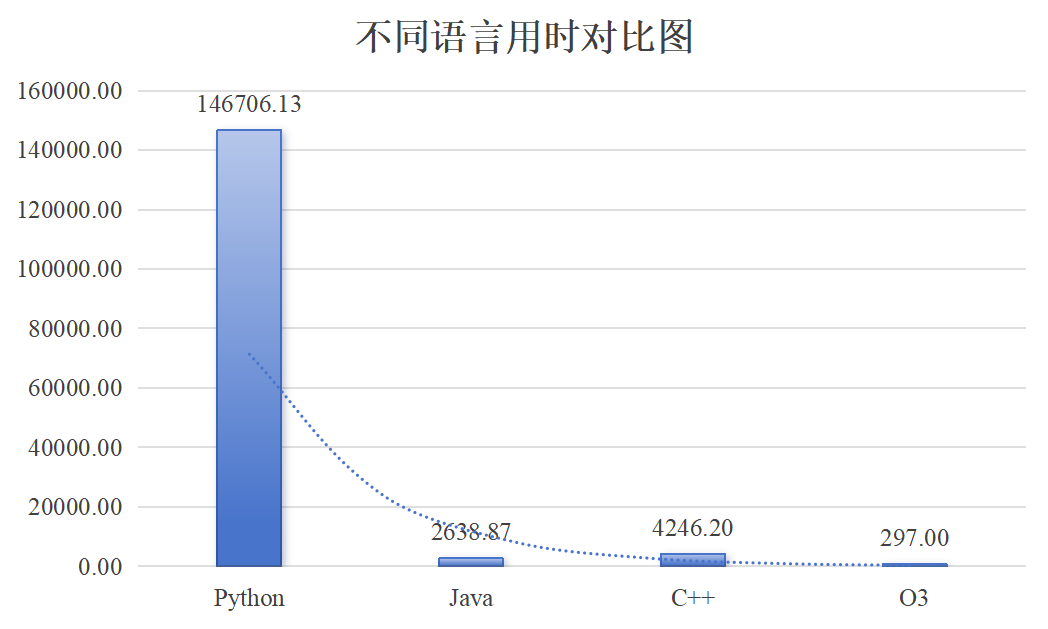
\includegraphics[height=.11\textheight]{./figure/Experience1_result1.png}
			\caption{不同语言用时对比图}
		\end{minipage}
		\begin{minipage}{.32\textwidth}
			\centering
			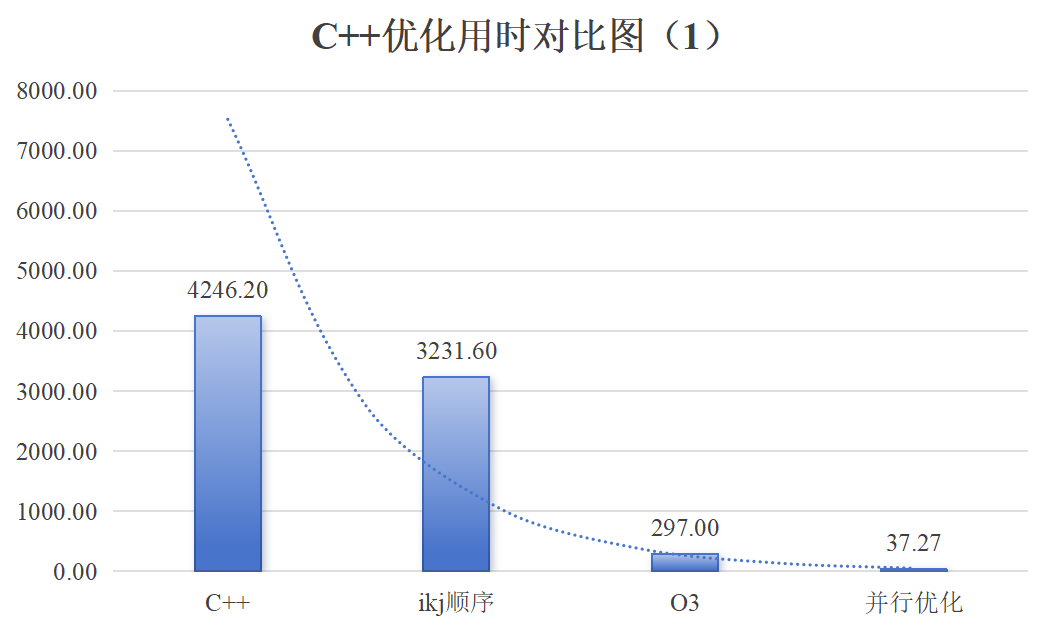
\includegraphics[height=.11\textheight]{./figure/Experience1_result2.png}
			\caption{C++优化用时对比图}
		\end{minipage}
		\begin{minipage}{.32\textwidth}
			\centering
			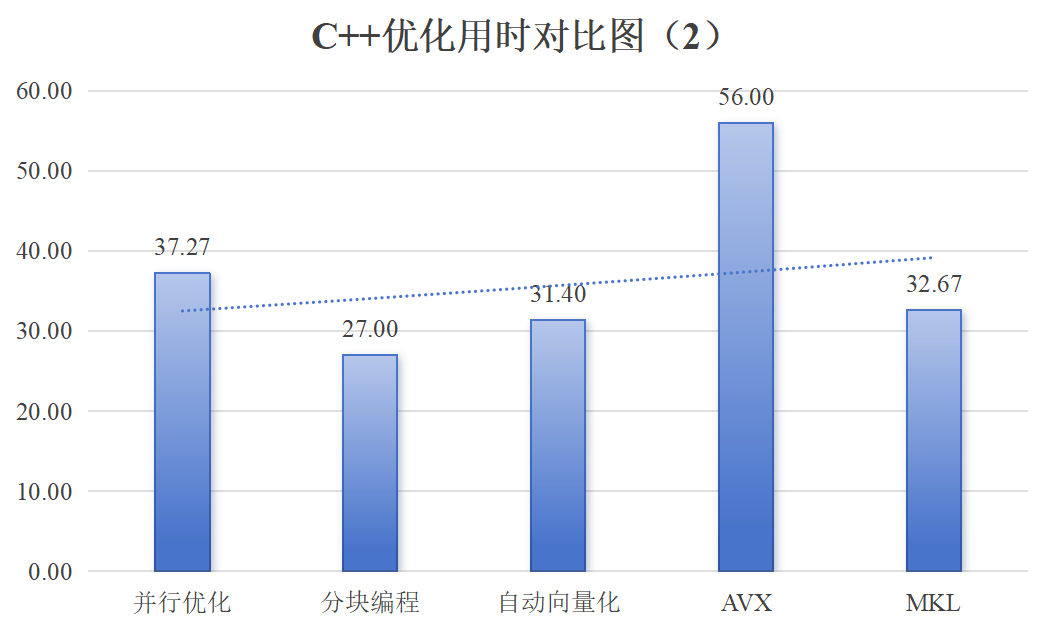
\includegraphics[height=.11\textheight]{./figure/Experience1_result3.png}
			\caption{C++优化用时对比图}
		\end{minipage}
	\end{figure}
	
	\subsubsection{实验1总结}
	
	实验结果表明,在不同的优化策略下,矩阵乘法的计算效率得到了显著提升。从最初的朴素 Python 代码(146706.13ms)到最终的分块优化(27.00ms),整体加速比达到了 5437.26 倍。其中,编译优化、多线程并行化及缓存优化是提升性能的关键因素,而向量化优化的效果受限于数据对齐和指令调度问题,需谨慎使用。
	
	此外,MKL 提供了一种便捷的高效计算方案,其性能虽然不及手工优化的最优方案,但对于通用应用场景,仍然是高效且易于集成的选择。
	
	\begin{table}[htbp]
		\centering	\small
		\caption{不同优化方法性能比对表}
		\vspace{-.75em}
		\begin{tabular}{m{.06\textwidth}<{\centering}|m{.17\textwidth}<{\centering}|m{.09\textwidth}<{\centering}|m{.11\textwidth}<{\centering}|m{.11\textwidth}<{\centering}|m{.11\textwidth}<{\centering}|m{.1\textwidth}<{\centering}}
			\toprule
			版本 & 实现描述 & 运行时间(ms) & 相对加速比 & 绝对加速比 & 浮点性能(GFLOPS) & 峰值性能百分比 \\
			\midrule
			1 & Python & 146706.13 & 1.00 & 1.00 & 0.015 & 0.001\% \\
			2 & Java & 2638.87 & 55.59 & 55.59 & 0.814 & 0.034\% \\
			3 & C++ & 4246.20 & 0.62 & 34.55 & 0.506 & 0.021\% \\
			4 & +调整循环顺序 & 3231.60 & 1.31 & 45.40 & 0.665 & 0.028\% \\
			5 & +编译优化 & 297.00 & 10.88 & 493.96 & 7.231 & 0.306\% \\
			6 & 并行化 & 37.27 & 7.97 & 3936.66 & 57.625 & 2.442\% \\
			7 & +分块乘法 & 27.00 & 1.38 & 5433.56 & 79.536 & 3.370\% \\
			8 & +自动向量化 & 31.40 & 0.86 & 4672.17 & 68.391 & 2.898\% \\
			9 & +手工AVX优化 & 56.00 & 0.56 & 2619.75 & 38.348 & 1.625\% \\
			10 & Intel\ MKL & 32.67 & 1.71 & 4491.00 & 65.739 & 2.786\% \\
			\bottomrule
		\end{tabular}
	\end{table}
	
	\subsection{单一优化方法在不同规模矩阵下的运行时间趋势}
	
	在第二组实验中,我们针对不同矩阵规模(从 $512 \times 512$ 到 $2048 \times 2048$)对不同语言及优化方法的运行时间进行了测试,以分析矩阵大小对计算性能的影响。实验结果表明,随着矩阵规模的增大,不同方法的运行时间表现出了不同的增长趋势
	
	\subsubsection{Python、Java 与 C++ 的基准性能对比}
	
	在未进行优化的情况下,Python、Java 和 C++ 三种语言的矩阵乘法计算都呈现出 近似 $O(n^3)$ 的增长趋势,符合三重循环算法的时间复杂度预测。然而,具体性能表现因语言实现方式的不同而有所差异:
	
	\begin{itemize}[itemsep=4pt, topsep=2pt, parsep=2pt]
		\item Python 运行时间远大于 Java 和 C++,并且随着矩阵规模的增长,运行时间的增长幅度更为显著。例如,512 规模矩阵的计算耗时 11,606 ms,而 2048 规模的计算耗时已达到 1,025,296 ms,即增长了 约 88 倍。这种较差的性能表现主要归因于 Python 采用解释执行方式,导致计算效率低下。
		\item Java 在小规模矩阵计算时与 C++ 性能接近,但在大规模矩阵下表现优于未经编译优化的 C++。例如,在 1024 规模矩阵下,Java 仅耗时 1,986 ms,而 C++ 需要 3,393 ms。这是因为 Java 采用了 JIT(Just-In-Time)编译技术,能够对热点代码进行优化,从而在运行时提高性能。
		\item C++ 在未进行编译优化时,整体性能虽优于 Python,但未能完全发挥其优势,特别是在大规模矩阵计算时,Java 甚至在部分规模上优于 C++(如 1920 规模时,Java 仅需 18,666 ms,而 C++ 需要 33,363 ms)。但在进行了编译优化后,C++ 性能大幅提升,远超 Java 和 Python。
	\end{itemize}
	
	\subsubsection{逐步优化的影响分析}
	
	在实验过程中,随着优化方法的逐步引入,矩阵乘法的计算时间整体呈现 下降趋势,同时其增长趋势也发生了变化。
	
	最初,ikj 顺序优化 通过调整循环顺序改善了缓存局部性,使得运行时间有所降低,但整体仍然保持 $O(n^3)$ 的增长趋势。随后,编译优化 的引入显著减少了计算时间,其增长趋势相较于未经优化的代码有所放缓。并行化编程 进一步利用了多核 CPU 计算资源,使得运行时间的增长速度明显降低,趋向于 次线性增长。在此基础上,分块编程 进一步优化了缓存利用率,优化效果略优于并行化方法。
	
	在向量化优化方面,自动向量化 通过 SIMD 指令优化了数据处理,进一步降低了计算时间,但在更大规模矩阵时,其优化效果有所减弱。相比之下,AVX 指令优化 试图通过手动编写 SIMD 指令提升性能,但实验结果表明其效果未能完全优于自动向量化,可能受到代码实现方式的影响。最终,MKL 优化 充分利用了 Intel 提供的数学库,实现了最优的计算性能,且在不同矩阵规模下均保持稳定的增长趋势,展现出极高的优化效果。
	
	\begin{figure}
		\captionsetup{font={small}}
		\begin{minipage}{.32\textwidth}
			\centering
			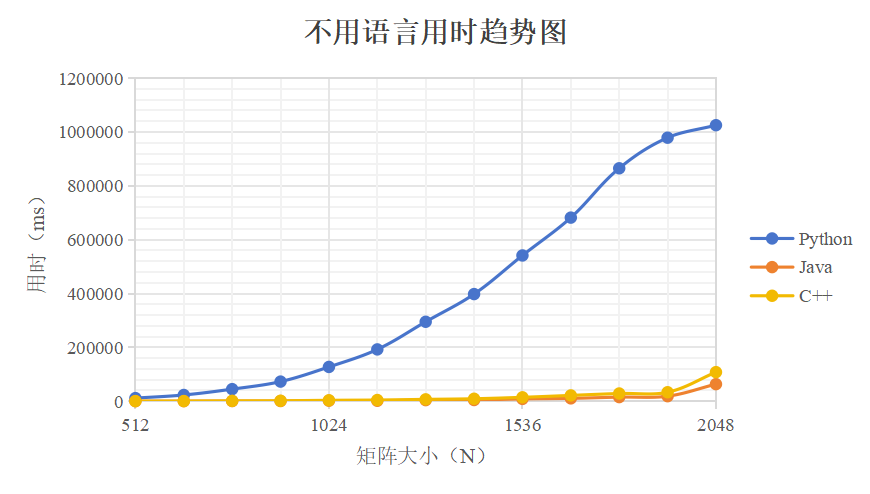
\includegraphics[height=.11\textheight]{./figure/Experience2_result1.png}
			\caption{不同语言用时趋势图}
		\end{minipage}
		\begin{minipage}{.32\textwidth}
			\centering
			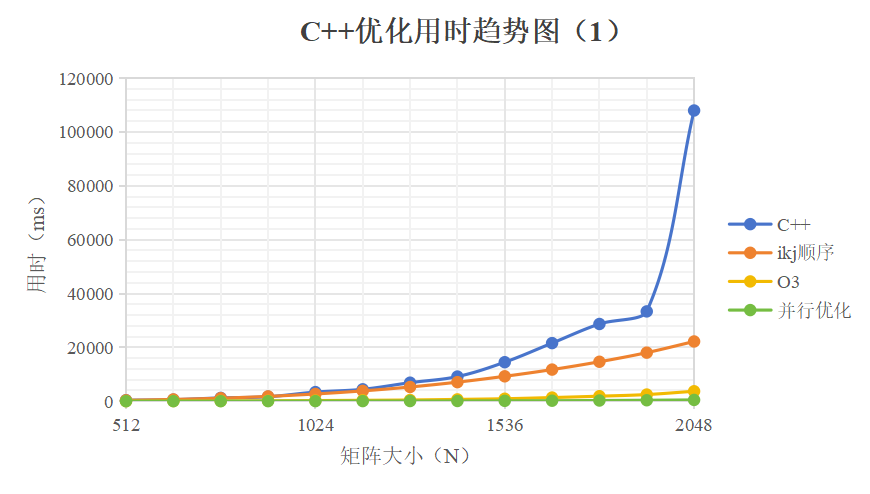
\includegraphics[height=.11\textheight]{./figure/Experience2_result2.png}
			\caption{C++优化用时趋势图}
		\end{minipage}
		\begin{minipage}{.32\textwidth}
			\centering
			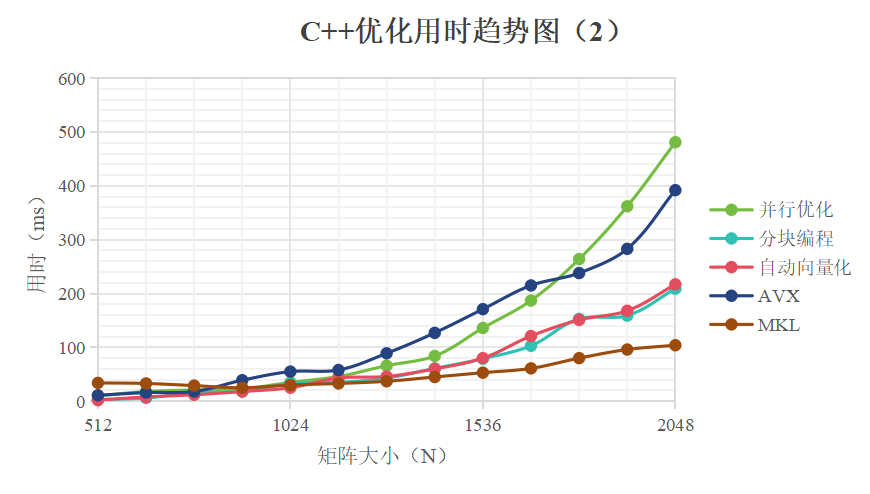
\includegraphics[height=.11\textheight]{./figure/Experience2_result3.png}
			\caption{C++优化用时趋势图}
		\end{minipage}
	\end{figure}
	
	\subsubsection{实验2总结}
	
	综上所述,矩阵乘法的计算时间随优化程度的提升逐步减少,增长趋势也由最初的 $O(n^3)$ 逐渐向次线性甚至接近 常数级别 变化。不同优化方法在不同矩阵规模下的影响有所差异,其中 MKL 优化 由于对硬件架构的深度适配,展现出了最佳的计算性能。综合考虑计算效率与适用范围,建议在实际应用中优先采用 MKL 优化 或结合 自动向量化与分块编程 的优化策略,以最大化提升矩阵乘法的计算效率。
	
	\section{总结与思考}
	
	本实验围绕环境配置与串行矩阵乘法优化展开,系统性地分析了不同优化策略对计算性能的影响。实验结果表明,朴素的三重循环矩阵乘法由于缓存未命中率高,计算效率较低。通过调整循环顺序(ikj 变换)、编译优化(-O3 选项)、并行化(OpenMP)、分块矩阵乘法、自动向量化及 Intel MKL 库优化,计算效率得到了显著提升。其中,编译优化能够大幅减少指令执行开销,并行化编程有效利用多核资源,分块矩阵乘法提高了缓存利用率,而 MKL 库则提供了接近理论峰值的性能表现。
	
	实验表明,合理选择优化策略能够极大提升矩阵运算的计算效率。在未来工作中,可进一步探索 GPU 加速(如 CUDA、OpenCL)、混合并行计算(MPI + OpenMP)以及更先进的硬件优化策略,以充分挖掘计算资源的潜能,提高矩阵计算在科学计算和工程应用中的实际可用性。
	
	\let\cleardoublepage\clearpage
	
	\begin{thebibliography}{99}  
		\bibitem{ref1} 彼得·S·帕切科,\ 马修·马伦塞克.\ 并行程序设计导论[M].\ 黄智濒,\ 肖晨\ 译.\ 原书第2版.\ 北京:机械工业出版社,\ 2024.
		\bibitem{ref2} 黄聃.\ 课件1[EB/OL].\ [2025-3-10].\ https://easyhpc.net/course/221/lesson/1412/material/3056.
	\end{thebibliography}
	
\end{document}
